\subsection{Logistic Regression}\label{ssec:logreg}

Logistic regression \cite{mckelvey1975statistical} is a well-known machine learning technique used in classification problems. This model can be implemented when classifying instances \cite{timmerman2005logistic} into dichotomous outcome like the problem being tackled in this project. Moreover, this model is also used in classification problems with non-binary outcomes \cite{debella2009spatial} and it is usually referred to as multinomial or “one vs rest” Logistic Regression. Although this model can be tweaked to classify multiple classes, in this project it will be utilized to classify a binary outcome (bankrupt or non-bankrupt). In this model the Logistic Sigmoid Function \eqref{eq:sigmoid} is used as a Hypothesis Function \eqref{eq:loghyp} to map an instance/s denoted as \(x\), with some given weights denoted as \(\theta\), to its Estimated Probability \eqref{eq:logprob} of the discrete outcome. Therefore, this function will output \(0 \leq h_\theta(x) \leq 1 \) as it is shown in Figure \ref{fig:log_func}. 
\begin{figure}[H]
\centering
  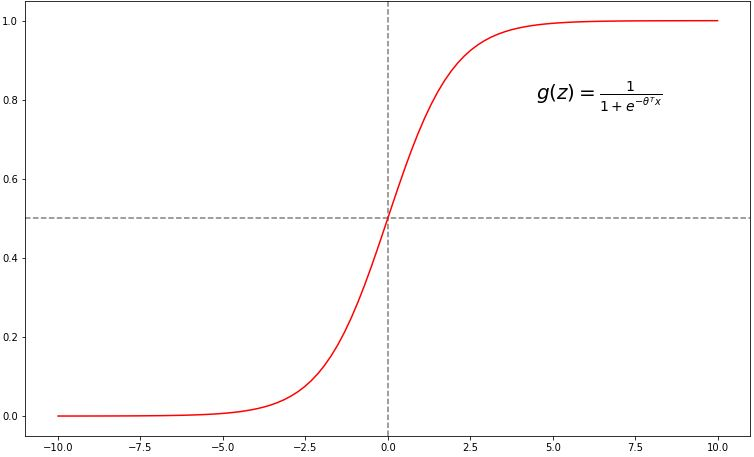
\includegraphics[scale = 0.5]{imgs/sigmoid_function.JPG}
  \caption{Logistic Sigmoid Function}
  \label{fig:log_func}
\end{figure}
\noindent Basically, the Hypothesis Function \eqref{eq:loghyp} will classify an instance/s to its predicted outcome.  Now since the function will output the estimated probability of the discrete outcome, the model needs to interpret this output to be able to classify into 0 or 1. To do so a decision boundary is needed to predict \(\hat{y} = 0 \ or\ \hat{y} = 1 \). In Condition \eqref{eq:logboundary} it is shown that  \(\hat{y} = 1\) if \(\ h_\theta(\theta^T x) \geq 0.5 \) and \(\hat{y} = 0\) if \(\ h_\theta(\theta^T x) < 0.5 \). Although in most cases the threshold is set to 0.5 as explained in Condition \eqref{eq:logboundary}, in other cases this may have to be adjusted to get better results depending on the problem being tackled (threshold must always be a value between 0 and 1). The decision boundary is a property of the hypothesis, so you can have non-linear decision boundaries by adding higher polynomial terms to the features.
\begin{multicols}{2}
    \begin{equation} \label{eq:sigmoid}
        g(z) = \frac{1}{1 + e^{-z}}
    \end{equation} 
    \\
    \begin{equation} \label{eq:loghyp}
        \begin{aligned}
            h_\theta = g(\theta^Tx)\\[0.1cm]
            h_\theta = \frac{1}{1 + e^{-g(\theta^Tx)}}
        \end{aligned}
    \end{equation}
\end{multicols}
\begin{multicols}{2}
\begin{equation} \label{eq:logprob}
    \begin{aligned}
        P=(\hat y = 0 | x;\theta) + P=(\hat y = 1 | x;\theta) = 1 \\[0.1cm]
        P=(\hat y = 0 | x;\theta) = 1 - P = (\hat y = 1 | x;\theta)
    \end{aligned}
\end{equation}
\\
\begin{equation} \label{eq:logboundary}
    \hat{y} = \begin{cases} 1 & \sigma(\theta^Tx) \geq 0.5 ; \theta^Tx \geq 0 \\ 0 & \sigma(\theta^Tx) < 0.5 ; \theta^Tx < 0 \end{cases}
\end{equation}
\end{multicols}
\noindent Now that the hypothesis is defined, and the classification function is explained the model must be trained to adjust its weights \(\theta\) to minimize the cost. The cost function \(J(\theta)\) utilized in Logistic Regression is shown in Equation \eqref{eq:logcost} and this cost function is used over the squared cost function to be able to find the global minimum when applying gradient descent (since it’s a convex cost function when using the Logistic Sigmoid Function). A desirable property of \(J(\theta)\) is that it greatly penalizes wrong predictions which have high probability with a high cost as shown in Figure \ref{fig:log_cost_0_1}. 
\begin{equation} \label{eq:logcost}
    \begin{aligned}
        Cost(h_\theta(x), y) = \begin{cases} y = 1 & -\log(h_\theta(x)) \\ y = 0 & -\log(1 - h_\theta(x)) \end{cases}
        \\
        J(\theta) = - \frac{1}{m} \sum\limits_{i=1}^{m} {Cost(h_\theta(x_i), y_i)}
        \\
        {J(\theta)} = - \frac{1}{m} \sum\limits_{i=1}^{m} {y_i \log h_\theta(x_i) + (1 - y_i) \log(1 - h_\theta(x_i))}
    \end{aligned}
\end{equation}
\begin{figure}[H]
\centering
  \begin{subfigure}[b]{0.35\textwidth}
    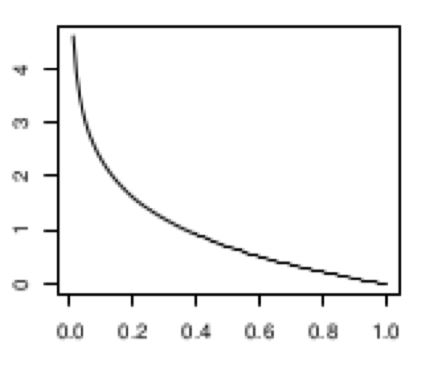
\includegraphics[scale = 0.5]{imgs/logistic_cost_1.JPG}
    \caption{y = 1}
    \label{fig:log_cost_1}
  \end{subfigure}
  %
  \begin{subfigure}[b]{0.35\textwidth}
    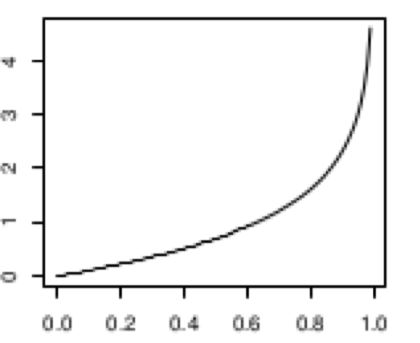
\includegraphics[scale = 0.52]{imgs/logistic_cost_2.JPG}
    \caption{y = 0}
    \label{fig:log_cost_2}
  \end{subfigure}
  \caption{Logistic Regression cost function}
  \label{fig:log_cost_0_1}
\end{figure}
\noindent Then the weights \(\theta\) are adjusted to minimize the cost function \(J(\theta)\) using gradient descent as shown in Equation \eqref{eq:loggradient}, until a termination condition is met. The termination condition is usually set to terminate when the number of max epochs is reached or when the step size \(\epsilon\) (the difference in cost after one epoch) has reach a certain threshold. The \(\alpha\) parameter usually referred to as the learning rate is the gradient decent step rate for each iteration which can be fixed or varied to control the steps at each iteration.   
\begin{equation} \label{eq:loggradient}
    \begin{aligned}
        \substack{minimize \\ \theta } {J}(\theta)\\[0.1cm]
        \theta_j := \theta_j - \alpha \frac{\partial}{\partial \theta_j} {J}(\theta)
    \end{aligned}
\end{equation}

\noindent In the training phase the gradient descent equation is applied for every weight \(\theta_j\) including the bias \(\theta_0\) until it converges or a termination condition is met, thus it will be adjusting weights \(\theta_j\) to minimize the cost \(J(\theta)\). There are other techniques which can be used to minimize \(J(\theta)\) such as Newton-Raphson, Conjugate Gradient, BFGS and L-BFGS. Once the model is trained it uses the hypothesis/classification function with the adjusted \(\theta_j\) to classify/predict unforeseen instances. 

\noindent Regularization is sometimes used to decrease the complexity, where the most commonly used regularization methods being Lasso/L1, and Ridge/L2 regularization. In Lasso Regularization a penalty term which sums up the magnitude of all coefficients except the bias \(\theta_0\), and then scaled by parameter \(\lambda\) is added to \(J(\theta)\) as shown in Equation \eqref{eq:l1}. In Ridge Regression a penalty term which sums up the square of all coefficients except the bias  \(\theta_0\), and then scaled by parameter  \(\lambda\) is added to \(J(\theta)\) as shown in Equation \eqref{eq:l2}.
\begin{equation} \label{eq:l1}
          {J(\theta)} = - \frac{1}{m} \sum\limits_{i=1}^{m} {y_i \log h_\theta(x_i) + (1 - y_i) \log(1 - h_\theta(x_i)) + \underbrace{\lambda \sum\limits_{j=1}^{n} |\theta_j|}_\text{L1}} 
\end{equation}
\begin{equation} \label{eq:l2}
          {J(\theta)} = - \frac{1}{m} \sum\limits_{i=1}^{m} {y_i \log h_\theta(x_i) + (1 - y_i) \log(1 - h_\theta(x_i)) + \underbrace{\lambda \sum\limits_{j=1}^{n} \theta_j ^2}_\text{L2}} 
\end{equation}